% Unofficial Yale Poster template.
% A fork of the UMich template https://www.overleaf.com/latex/templates/university-of-michigan-umich-poster-template/xpnqzzxwbjzc
% which is fork of the MSU template https://www.overleaf.com/latex/templates/an-unofficial-poster-template-for-michigan-state-university/wnymbgpxnnwd
% which is a fork of https://www.overleaf.com/latex/templates/an-unofficial-poster-template-for-new-york-university/krgqtqmzdqhg
% which is a fork of https://github.com/anishathalye/gemini
% also refer to https://github.com/k4rtik/uchicago-poster



\documentclass[final]{beamer}

% ====================
% Packages
% ====================

\usepackage[T1]{fontenc}
\usepackage{lmodern}
\usepackage[size=custom, width=122,height=91, scale=1.2]{beamerposter}
\usetheme{gemini}
\usepackage{svg}
\usecolortheme{msu}
\usepackage{graphicx}
\usepackage{booktabs}
\usepackage{tikz}
\usepackage{pgfplots}
\pgfplotsset{compat=1.14}
\usepackage{anyfontsize}
\usepackage{xcolor}
\definecolor{myHighlight}{RGB}{0,130,120}
\definecolor{myDarkRed}{RGB}{180, 20, 20}
\definecolor{myDarkGreen}{RGB}{0, 100, 40}
\setbeamercolor{caption name}{fg=black}

% ====================
% Lengths
% ====================

% If you have N columns, choose \sepwidth and \colwidth such that
% (N+1)*\sepwidth + N*\colwidth = \paperwidth
\newlength{\sepwidth}
\newlength{\colwidth}
\setlength{\sepwidth}{0.025\paperwidth}
\setlength{\colwidth}{0.3\paperwidth}

\newcommand{\separatorcolumn}{\begin{column}{\sepwidth}\end{column}}

% ====================
% Title
% ====================

\title{
  \resizebox{0.55\paperwidth}{!}{Diffusion Policy: Visuomotor Policy Learning via Action Diffusion}
}

% 2. YOUR NAMES:
\author{Yacine Khalil \& Iliass Khoutaibi}

% 3. SUBTITLE (Original Authors):
% We use \institute to place this text right below your names.
\institute{
  \large \textit{Based on the original paper by Cheng Chi, Zhenjia Xu, Siyuan Feng, Eric Cousineau, Yilun Du, Benjamin Burchfiel, Russ Tedrake \& Shuran Song}
}

% ====================
% Footer
% ====================

\footercontent{
  \noindent
  \begin{tabular*}{\paperwidth}{@{\hspace{1.5cm}} l @{\extracolsep{\fill}} c @{\extracolsep{\fill}} r @{\hspace{1.5cm}}}
    
    {\bfseries
    \href{https://github.com/KHOUTAIBI/DiffusionPolicy}{github.com/KHOUTAIBI/DiffusionPolicy}
    }
    
    &
    
    {\bfseries
    11 December 2025 \;|\; Inria Paris (48 rue Barrault)
    }
    
    &
    
    {\bfseries
    \href{mailto:yacine.khalil@telecom-paris.fr}{yacine.khalil@telecom-paris.fr}
    \quad
    \href{mailto:iliass.khoutaibi@telecom-paris.fr}{iliass.khoutaibi@telecom-paris.fr}
    }
    
  \end{tabular*}
}




% ====================
% Logo (optional)
% ====================

% use this to include logos on the left and/or right side of the header:
% Left: institution
\logoright{
    
\includegraphics[height=5.5cm]{figures/QR_code.pdf}
    \hspace{0.4cm}
    
\includegraphics[height=5.5cm]{logos/Logo_Télécom_ParisTech.pdf}
}
% Right: funding agencies and other affilations 
\logoleft{
\includegraphics[height=6cm]{logos/MVA.pdf}}
% ====================
% Body
% ====================

\begin{document}

\begin{frame}[t]
\begin{columns}[t]
\separatorcolumn


\begin{column}{\colwidth}

\vspace{-1cm}
\begin{alertblock}{Objectives}

  \begin{itemize}
    \item \textbf{Visuomotor Policy as a Diffusion Process}: Reformulate robot policy learning as a conditional denoising diffusion process on the action space
    
    \item \textbf{Capture Multimodality \& Stability}: Overcome the limitations of Explicit Policies and IBC by naturally modeling multimodal action distributions with stable training dynamics
    
    \item \textbf{Action Sequence Prediction}: Leverage the scalability of diffusion models to predict high-dimensional action sequences, ensuring temporal consistency and smoothness.

    \item \textbf{Evaluate Architectures}: Systematically benchmark CNN-based and Transformer-based backbones across challenging tasks like Push-T and Franka Kitchen

    \item \textcolor{myHighlight}{\textbf{Project main contribution}: \textbf{Investigate Flow Matching} as a deterministic alternative to Diffusion in order to improve inference speed.}

    \end{itemize}

\end{alertblock}

\begin{block}{Introduction}

\textbf{Diffusion Policy} reformulates visuomotor control as a \emph{conditional denoising diffusion process} in the action space, enabling expressive and stable policy learning.

\vspace{0.5em}

\begin{columns}
    \begin{column}{0.48\linewidth}
        \textcolor{myDarkRed}{\textbf{Problems Addressed:}}
        \begin{itemize}
            \item \textbf{Multimodality:} Standard policies (MSE loss) average multiple valid trajectories into a single, invalid action (e.g., going between two obstacles rather than around one).
            \item \textbf{Training Instability:} Implicit behavior cloning (EBMs) requires negative sampling and is difficult to optimize.
            \item \textbf{Temporal Consistency:} Single-step predictors often result in jittery motion.
        \end{itemize}
    \end{column}
    
    \begin{column}{0.48\linewidth}
        \textcolor{myDarkGreen}{\textbf{Key Idea:}}
        \begin{itemize}
            \item Instead of outputting actions directly, the policy learns the \emph{gradient of the data distribution} (score function).
            \item It progressively denoises random gaussian noise into a coherent action sequence $ \mathbf{A}_t $.
        \end{itemize}
        
        \vspace{0.5em}
        \textcolor{myHighlight}{\textbf{Outcome:}} \textbf{+46.9\%} average success rate across 15 benchmarks compared to LSTM-GMM and BET.
    \end{column}
\end{columns}

\vspace{0.5em}

\begin{figure}
    \centering
    % The fcolorbox adds a white background behind the image to fix the contrast issue
    \setlength{\fboxsep}{2pt} % Optional: small padding around image
    \setlength{\fboxrule}{0pt}
    \fcolorbox{white}{white}{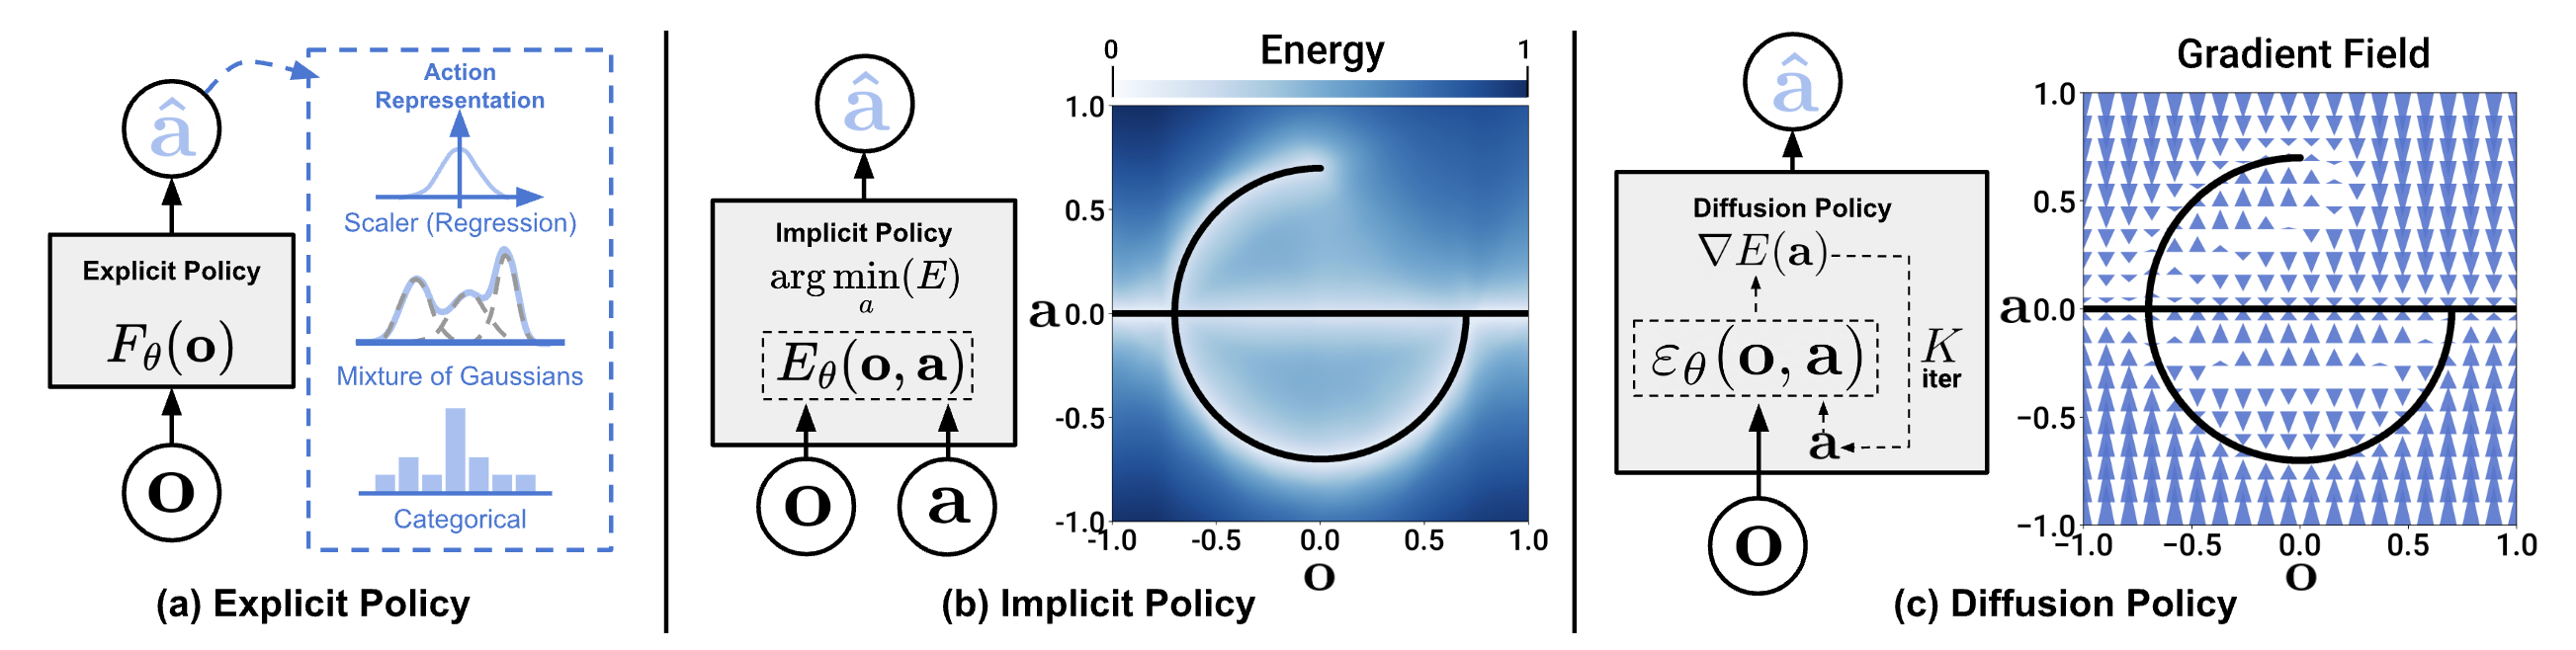
\includegraphics[width=1.0\linewidth]{figures/teaser.png}}
    
    % Restored Caption
    \caption{Comparison of policy representations. Diffusion Policy (right) denoises random actions through a learned gradient field.}
    \label{fig:teaser}
\end{figure}

\end{block}


\begin{block}{Receding Horizon Control (RHC)}

    Unlike standard policies that predict a single step, Diffusion Policy predicts a \textbf{sequence} of actions $\mathbf{A}_t = \{\mathbf{a}_t, \dots, \mathbf{a}_{t+h}\}$.
    
    \vspace{0.3em}
    
    \textbf{Execution Strategy:}
    We execute only the first $m$ steps of the predicted trajectory ($m < h$) before replanning based on the latest observation $\mathbf{O}_t$.
    
    \vspace{0.3em}
    
    This rapid replanning creates a \textbf{high-frequency feedback loop} (Loop Closure) that effectively rejects physical disturbances, while the sequence prediction ensures smooth, non-jittery motion.

\end{block}

\end{column}

\separatorcolumn

\begin{column}{\colwidth}
\vspace{-1cm}
\begin{block}{Theoretical Background}

\textbf{1. Why Diffusion?}  
- Implicit policies model the action distribution with an Energy-Based Model (EBM):  
\[
p(\mathbf{a}|\mathbf{o}) \propto e^{-E(\mathbf{o}, \mathbf{a})}.
\]  
- Direct minimization of $E$ is often unstable.

\vspace{0.5em}

\textbf{2. Diffusion as Score Matching}  
- Instead of learning $E$ directly, learn the \emph{score function}:
\[
\nabla_{\mathbf{a}} \log p(\mathbf{a}|\mathbf{o}) = -\nabla_{\mathbf{a}} E(\mathbf{o}, \mathbf{a})
\]  
- Conceptually, this is equivalent to learning how to "denoise" a latent action variable $\mathbf{A}^k$ over $K$ steps.

\vspace{0.5em}

\begin{minipage}[t]{0.48\linewidth}
    \textbf{Training (Noise Prediction)}\\[0.3em]
    - Network $\varepsilon_\theta$ predicts noise added to $\mathbf{A}^0$.  
    - Loss:
    \[
    \mathcal{L} = \text{MSE}\Big( \varepsilon, \; \varepsilon_\theta(\mathbf{A}^k, k, \mathbf{O}) \Big)
    \]  
    - Forward model of noisy action:
    \[
    \mathbf{A}^k = \sqrt{\bar{\alpha}_k}\mathbf{A}^0 + \sqrt{1-\bar{\alpha}_k}\varepsilon
    \]  
\end{minipage}%
\hfill
\vrule width 0.5pt % thin vertical line
\hfill
\begin{minipage}[t]{0.48\linewidth}
    \textbf{Inference (Iterative Denoising)}\\[0.3em]
    - Start from Gaussian noise: $\mathbf{A}^K \sim \mathcal{N}(0, I)$.
    - Iteratively refine the action:
    \[
    \mathbf{A}^{k-1} = \alpha_k (\mathbf{A}^k - \gamma_k \varepsilon_\theta(\mathbf{A}^k, k, \mathbf{O}_t)) + \sigma z
    \]
    \textcolor{myDarkRed}{$\rightarrow$ Requires $K$ forward passes!}
\end{minipage}

\end{block}

\vspace{-0.5cm}

\begin{block}{Training and Inference}

\textbf{(a) General Formulation}
- At timestep \( t \), the policy observes the last \( T_o \) frames \( \mathbf{O}_t \).
- It predicts a sequence of \( T_p \) future actions \( \mathbf{A}_t \) and executes \( T_a \) steps.

\vspace{0.3em}

\textbf{(b) CNN-based Diffusion Policy}  
- Observation encoding \( \mathbf{O}_t \) conditions all conv layers via \emph{FiLM}.  
- Start from noisy action \( \mathbf{A}^K_t \sim \mathcal{N}(0,I) \).  
- Noise-prediction network \( \varepsilon_\theta \) iteratively denoises over \( K \) steps → final action \( \mathbf{A}^0_t \).

\vspace{0.3em}

\textbf{(c) Transformer-based Diffusion Policy}  
- Observation embedding injected into each decoder block via cross-attention.  
- Action embeddings use causal self-attention → each token sees only itself + previous actions.  
- Ensures autoregressive consistency while conditioning on \( \mathbf{O}_t \).

\vspace{0.3em}

\begin{figure}[h!]
    \centering
    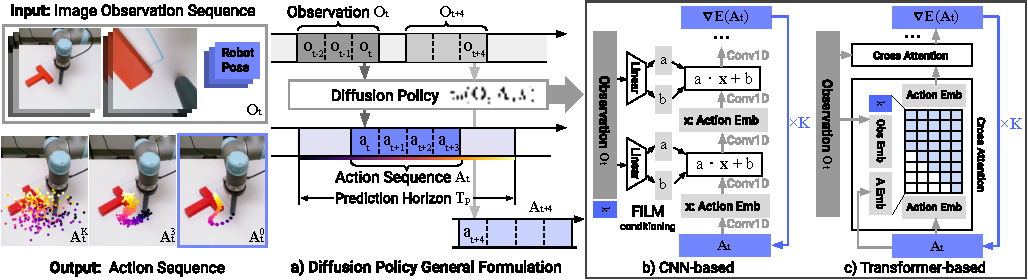
\includegraphics[width=0.95\linewidth]{figures/Figure_2.pdf}
    \caption{Diffusion policy network architecture}
\end{figure}

\end{block}
\vspace{-1.4cm}

\begin{block}{Testing on PushT task}
     We evaluated performance on the \textbf{PushT} benchmark, requiring precise multimodal pushing actions (going left vs. right).

     \vspace{0.3em}

     \begin{columns}[c] % [c] vertically centers all 3 images
        
        % --- 1. PushT Environment ---
        \begin{column}{0.28\linewidth}
            \centering
            % Increased internal width to 0.95 since the column itself is narrower
            
\includegraphics[width=0.95\linewidth]{figures/PushT.pdf}
            \vspace{0.2em} 
            \textbf{\footnotesize Env. Setup}
        \end{column}
        
        % --- 2. Multimodal Choice (NEW) ---
        \begin{column}{0.28\linewidth}
            \centering
            
\includegraphics[width=0.95\linewidth]{figures/multimodal_choice.pdf}
            \vspace{0.2em}
            \textbf{\footnotesize Multimodal Paths}
        \end{column}
        
        % --- 3. Loss Plot ---
        \begin{column}{0.40\linewidth}
            \centering
            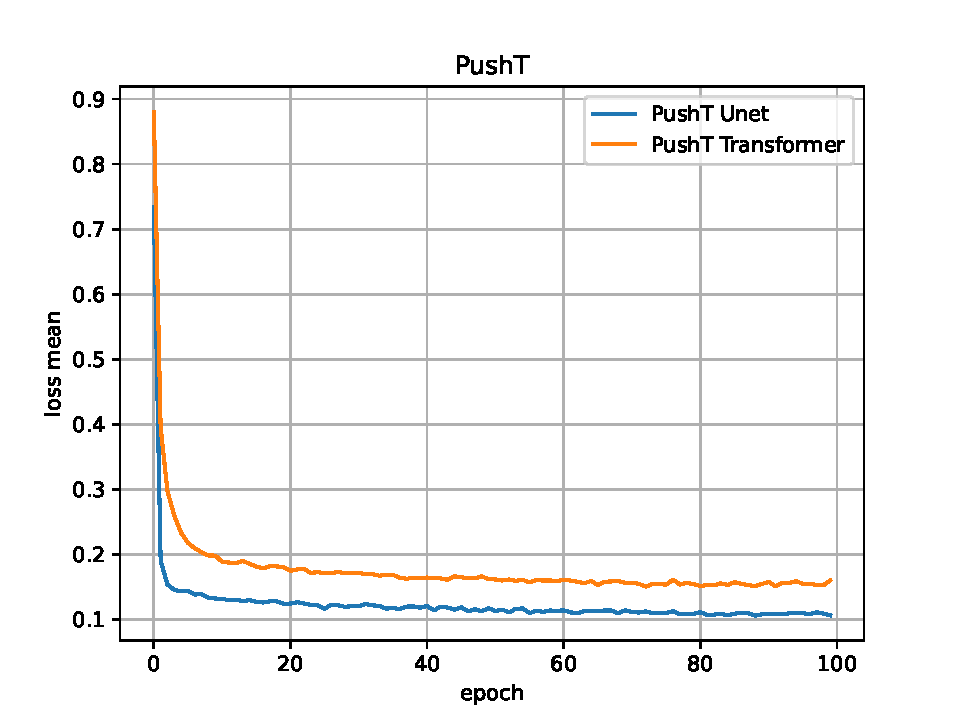
\includegraphics[width=0.95\linewidth]{figures/loss_pusht_unet_transformer.pdf}
            \vspace{0.2em}
            \textbf{\footnotesize Training Loss}
        \end{column}
        
     \end{columns}
\end{block}

\end{column}

\separatorcolumn

\begin{column}{\colwidth}
\vspace{-1cm}
\begin{block}{Testing on Franka Kitchen task}
     We evaluated performance on the \textbf{Franka Kitchen} benchmark, a challenging long-horizon task.

     \vspace{0.3em}

     \begin{columns}[c]
        % --- Left: Environment ---
        \begin{column}{0.4\linewidth}
            \centering
            
\includegraphics[width=0.6\linewidth]{figures/franka_kitchen.pdf}
            \vspace{0.2em}
        \end{column}
        
        % --- Right: Loss Plot ---
        \begin{column}{0.58\linewidth}
            \centering
            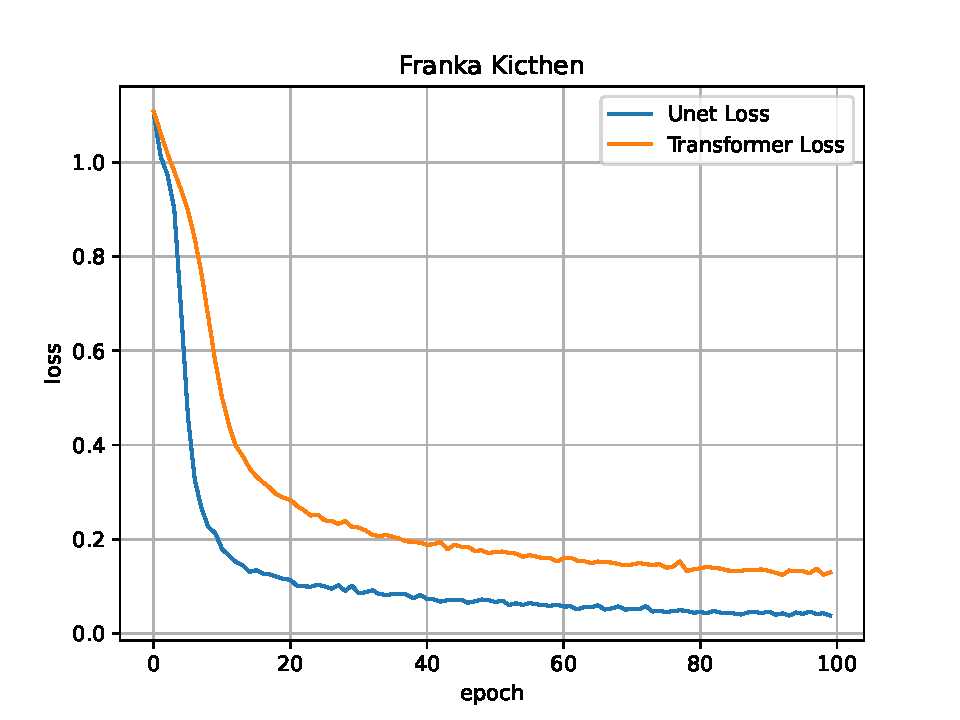
\includegraphics[width=0.65\linewidth]{figures/losses_unet_transformer.pdf}
            \vspace{0.2em}
        \end{column}
     \end{columns}
  \end{block}
\vspace{-1.4cm}
  \begin{block}{Diffusion Policy vs. Flow-matching Policy}

   \begin{figure}
       \centering
       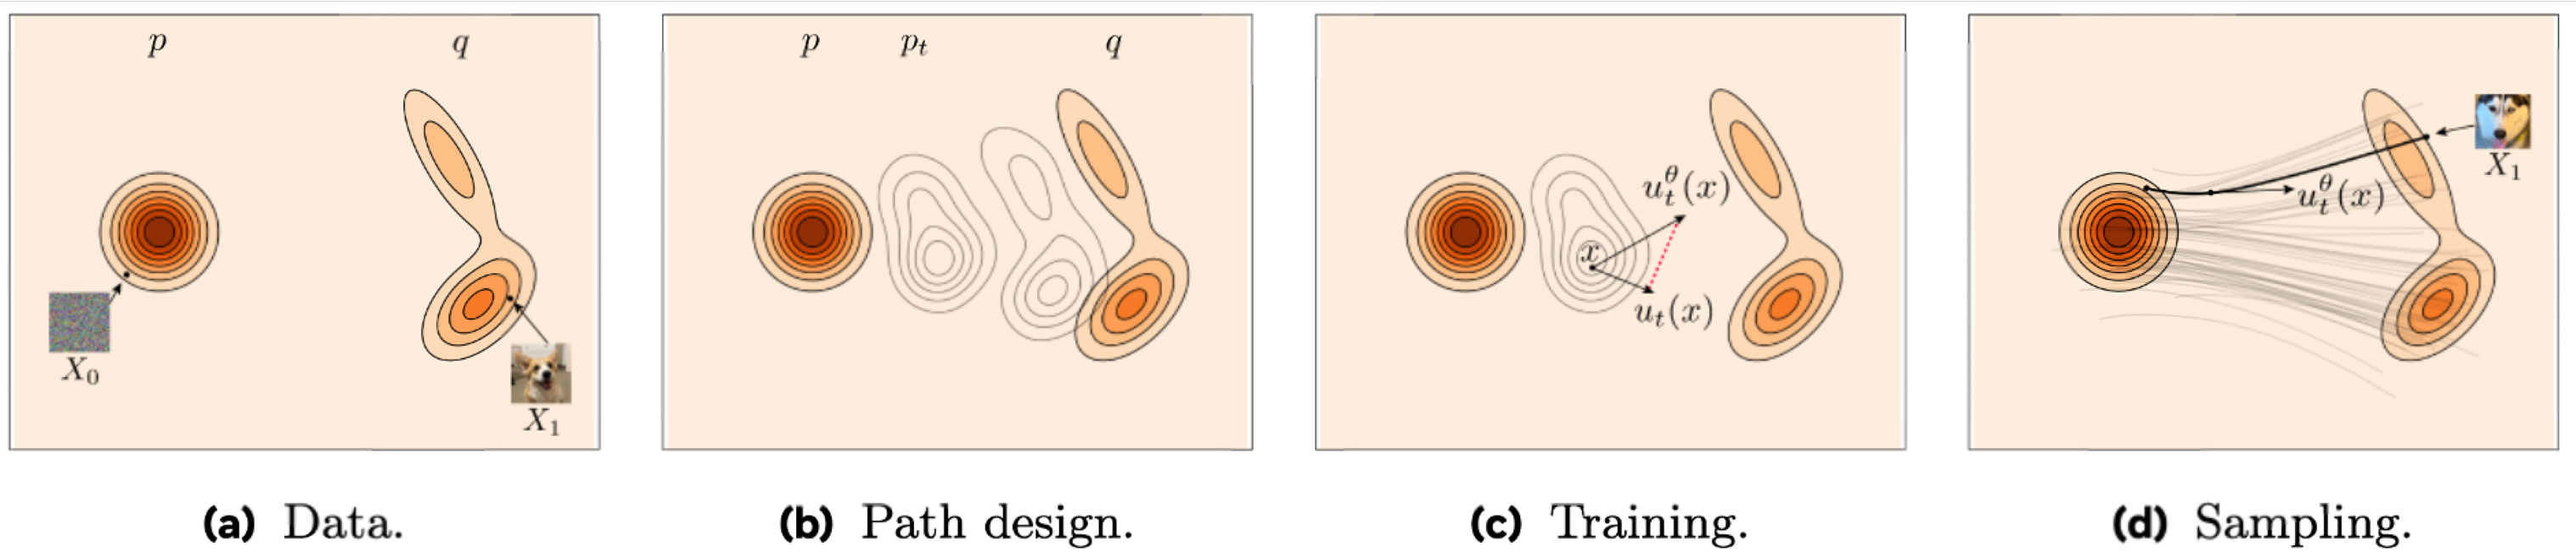
\includegraphics[width=1.0\linewidth]{figures/flow_matching.png}
       \caption{Concept of Flow-matching}
       \label{fig:enter-label}
   \end{figure}
    \vspace{-0.8cm}
    

    \begin{table}
      \centering
      \begin{tabular}{l r r c}
        \toprule
        \textbf{Denoising process} & \textbf{Task} & \textbf{Inference time} & \textbf{Std} \\
        \midrule
        DDPM & PushT & \textbf{1.2s} & 0.16s \\
        Flow matching & PushT & \textbf{1.01s} & 0.13s \\
        DDPM & Franka Kitchen & \textbf{8.02s} & 0.76s \\
        Flow matching & Franka Kitchen & \textbf{6.82s} & 0.64s \\
        \bottomrule
      \end{tabular}
      \caption{Successful inference time using both denoising methods on the benchmarks}
    \end{table}

  \end{block}
\vspace{-1.4cm}

\begin{block}{Conclusion \& Future Work}
    Diffusion Policy achieves state-of-the-art visuomotor control by modeling multimodal actions with strong temporal consistency. Its main limitation is the high latency caused by iterative denoising.

We show that \textbf{Flow Matching} offers a deterministic alternative, reducing inference time by $\approx \mathbf{15\%}$ on both benchmarks, with a slight drop in trajectory quality.

\textbf{Limitations \& Future Work:}
\begin{itemize}
    \item \textbf{Real-World Gap:} Inference remains too slow for reliable deployment despite the speedup.
    \item \textbf{No Exploration:} Unlike RL, the model does not explore the environment and relies solely on offline demonstrations.
\end{itemize}

  
  \end{block}

\vspace{-1.4cm}
    \begin{block}{References}
    \vspace{-0.2cm}
    \nocite{*}
    \footnotesize{\bibliographystyle{plain}\bibliography{poster}}
    
    \end{block}

\end{column}

\separatorcolumn
\end{columns}
\end{frame}
\end{document}
